\section{Subsistema: Controle} \label{sec:controle}

\par O subsistema responsável pelo controle do carrinho autônomo controlará os motores (que a princípio estarão acoplados às rodinhas traseiras do carrinho). Além disso, esses subsistema fará a leitura dos sensores responsáveis por localizar o cadeirante e evitar colisões. 

\par Como mostrado na Figura \ref{fig:esqCarrinho}, os sensores se comunicarão com o microcontrolador, que por sua vez processará tais sinais elétricos e, com base em um algoritmo embarcado no próprio microcontrolador, acionará os atuadores (motores). Ademais, existirá um controle remoto que o usuário pode utilizar para efetuar as funções de liga/desliga. A Figura \ref{fig:esqCarrinho} exibe uma vista superior esquemática do protótipo a ser desenvolvido:

% \begin{figure}
% \centering
% \begin{minipage}{.5\textwidth}
%   \centering
%   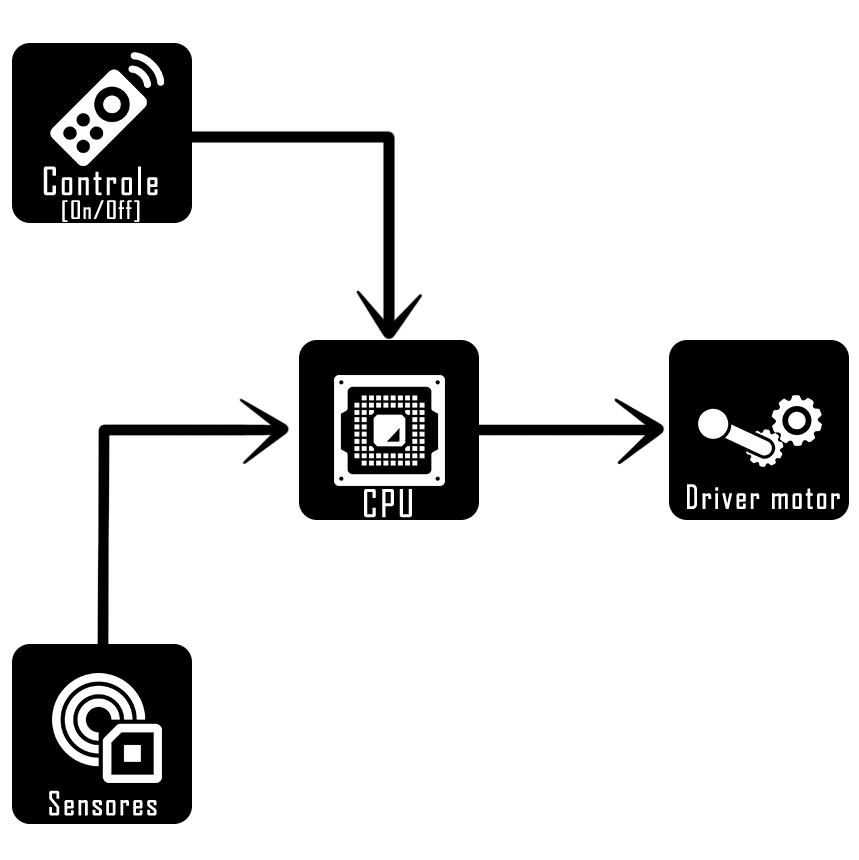
\includegraphics[width=.4\linewidth]{figuras/diagrama.png}
%   \captionof{figure}{Diagrama do sistema de controle do carrinho}
%   \label{fig:esqCarrinho}
% \end{minipage}%
% \begin{minipage}{.5\textwidth}
%   \centering
%   \includegraphics[width=.4\linewidth]{figuras/schematic.png}
%   \captionof{figure}{Vista superior esquemática do protótipo}
%   \label{fig:schematic}
% \end{minipage}
% \end{figure}

\begin{figure}[hb]
		\centering
		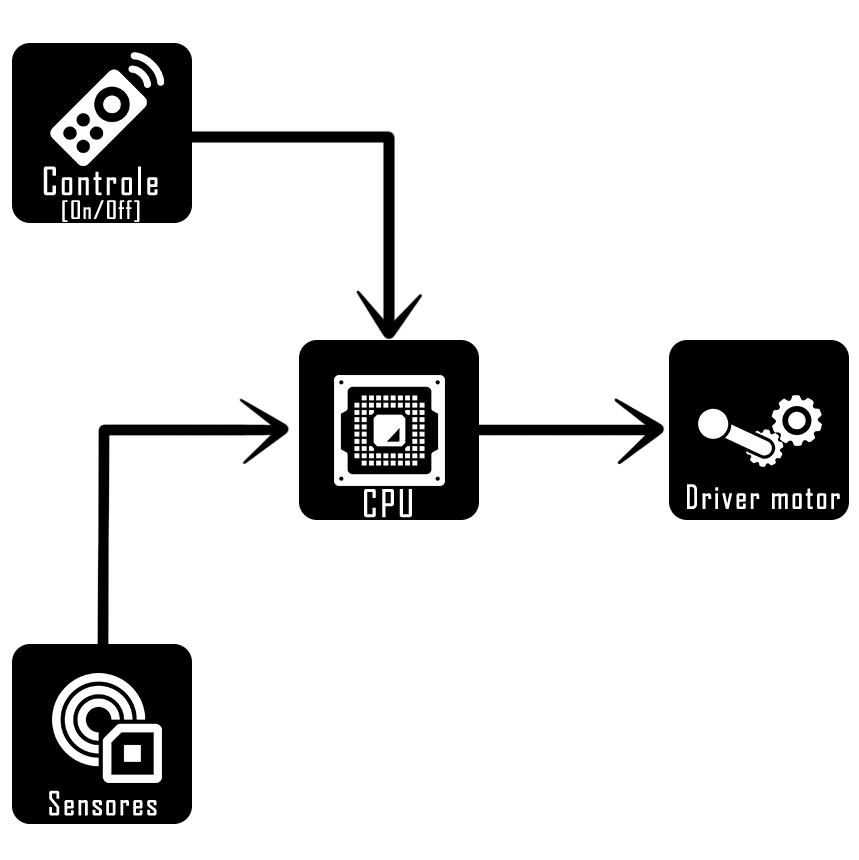
\includegraphics[width=.5\textwidth]{figuras/diagrama.png}
		\caption{Esquemático do sistema de controle do carrinho}
		\label{fig:esqCarrinho}
\end{figure} 

\newpage 
\begin{figure}[hb]
		\centering
		\includegraphics[width=.5\textwidth]{figuras/schematic.png}
		\caption{Vista superior esquemática do protótipo}
		\label{fig:schematic}
\end{figure} 



\subsection{Relatório de Pesquisa Técnica}
\par O subsistema responsável pelo controle do carrinho autônomo, a princípio, pode ser dividido em três outros subsistemas:

\begin{itemize} 
\item Sistema de locomoção do carrinho;
\item Sistema de localização do cadeirante;
\item Sistema anti-colisão.
\end{itemize}

\subsubsection{Sistema de Locomoção do Carrinho}

    \par Inicialmente, pretende-se usar dois motores DC, de forma que cada um esteja acoplado à um roda traseira do carrinho. O controle desses motores será feito por meio da técnica PWM (\textit{Pulse Width Modulation}), que consiste em manter a frequência de uma onda quadrada fixa e variar o tempo que o sinal fica em nível lógico alto (\textit{duty cycle}), isto é, essa técnica proporciona o controle da velocidade de rotação do motor \cite{mecaweb}:
					
$$
Duty \hspace{0.1 cm} Cycle \propto Rotação \hspace{0.1  cm} do \hspace{0.1 cm} motor
$$

\par Os motores DC ou de corrente continua são muito utilizados nas áreas de robótica, mecatrônica e automação.  Eles funcionam quando uma tensão é aplicada em seus terminais de alimentação. O sentido que o motor gira depende do sentido de circulação da corrente em seus enrolamentos, ou seja, a mudança de polaridade da alimentação implica na mudança de direção de rotação. 

\par O controle do sentido de rotação de um motor DC pode ser feito usando um circuito eletrônico conhecido como Ponte-H. Elas são fundamentais no controle direcional do motor e permitem que um microcontrolador, que fornece sinais de corrente relativamente baixa, controle a velocidade dos motores que exigem correntes elevadas através de pinos de PWM. \cite{newtoncbraga}: 

\subsubsection{Sistema de Localização do Cadeirante}

\par Para o sistema de localização do cadeirante, foram consideradas três tecnologias diferentes:

\begin{itemize}  
\item Localização baseada em emissão/recepção de ondas eletromagnéticas;
\item Processamento de imagem;
\item Emissão de luz infravermelha.
\end{itemize}

\par O método de localização do cadeirante por meio de emissão/recepção de ondas eletromagnéticas analisado \cite{min2015active} consiste em um sistema em que o alvo emite ondas eletromagnéticas através de uma antena omnidirecional,  
e o carrinho autônomo conta com uma antena direcional que continuamente escaneia o ambiente à procura do sinal emitido pelo alvo. Um esquemático de tal sistema é apresentado na Figura \ref{fig:antenaElectroMagWave}. 

\newpage

\begin{figure}[ht]
		\centering
		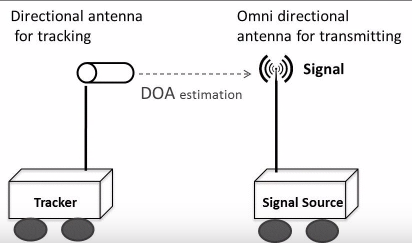
\includegraphics[width=.5\textwidth]{figuras/antenaElectroMagWave.png}
		\caption{Esquemático do sistema de controle do carrinho}
		\label{fig:antenaElectroMagWave}
	\end{figure} 
    

\par No sistema baseado em transmissão/recepção de ondas estudado, apenas uma antena direcional é empregada, de modo que a mesma varre o ambiente em ângulos obtusos de até 180$^{\circ}$. Uma desvantagem dessa implementação é que haveria um grande desgaste da estrutura mecânica que move a antena, uma vez que a estrutura que faz o escaneamento do ambiente se move de forma contínua durante todo o tempo de uso do protótipo. 

\par Estudou-se também um sistema baseado em processamento de imagem  \cite{isobe2014human} que consiste em detectar cores pré-determinadas, ou seja, o sistema é configurado de modo que uma determinada forma (com uma cor específica) seja isolado, e dessa forma, o sistema é capaz de identificar as mudanças de direção e distância do alvo através de detecção e análise das distorções nessa forma. É sabido, entretanto, que esse método de localização do alvo demanda uma ferramenta de maior poder de processamento. Sendo assim, microcontroladores mais simples como ATMega328, PIC32 e MSP430 não seriam as melhores opções para esse tipo de implementação.

\par Uma outra forma analisada de detectar a localização do cadeirante foi a desenvolvida por \cite{calcar} a qual emprega sensores infravermelhos de longo alcance para detectar a mudança de direção de um carrinho de controle remoto. Essa técnica, entretanto, requer que o alvo tenha uma superfície bem uniforme, em que as rajadas de luz infravermelha possam ser refletidas adequadamente. A Figura \ref{fig:IRbot} abaixo mostra como o sistema determinaria a condição de atuar sobre as rodas (se a diferença de distâncias lidas pelos sensores for maior que um determinado limiar $\epsilon$, então os atuadores são acionados e movem as rodas dianteiras).
\newpage
 
 \begin{figure}[ht]
		\centering
		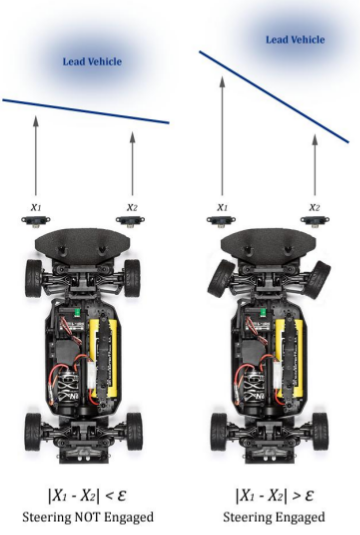
\includegraphics[width=.3\textwidth]{figuras/IRbot.png}
		\caption{Esquemático do sistema de controle do carrinho}
		\label{fig:IRbot}
	\end{figure} 

\par Após revisar e analisar os métodos supracitados, concluiu-se que, inicialmente a implementação do sistema de localização do cadeirante será abordada com uma combinação dos sistemas de detecção através de transmissão/recepção de ondas eletromagnéticas e de processamento de imagem. A estratégia é trabalhar com as duas frentes de forma paralela e ao fim, se possível, integrar as duas em um mesmo produto final. Caso não seja possível entregar as duas soluções integradas, espera-se que ao menos uma delas esteja completamente funcional e atendendo todos os requisitos funcionais e não funcionais do projeto. 

\subsubsection{Sistema de Anti-Colisão}
\par Esse sistema tem como principais objetivos:

\begin{itemize}
\item Manter uma determinada distância entre o usuário (cadeirante) e o carrinho,
\item Evitar as colisões com os objetos presentes no ambiente do supermercado
\end{itemize}

\par Tal sistema consistirá em um conjunto de sensores ultrassônicos os quais efetuam leituras de distâncias de 2 cm a 4 m com precisão de até 3 mm. O posicionamento de tais sensores será feito de uma forma em que seja possível  \cite{flipeflop}.

\subsection{Algoritmos}

\par Para a boa realização do projeto será necessário a integração de vários algoritmos específicos de cada problema encontrado. A partir de pesquisas preliminares chegamos a alguns possíveis candidatos a aplicação na solução final. Seguindo o fluxo do diagrama da Figura \ref{fig:diagramaAlg} é possível visualizar os principais blocos de processamento e quais algoritmos serão necessários para realização de cada etapa.

\begin{figure}[ht]
	\centering
	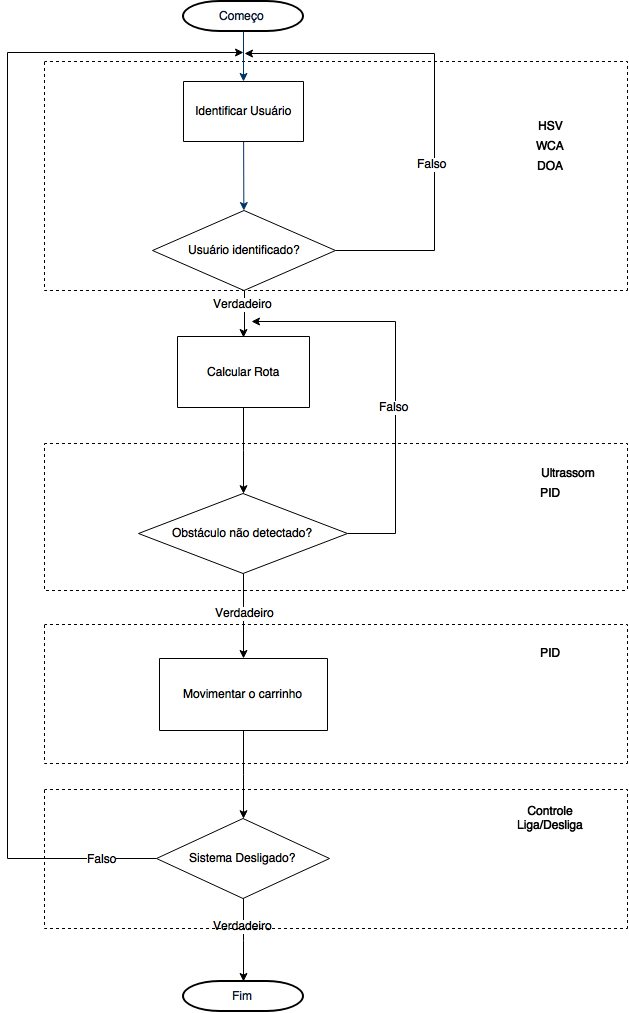
\includegraphics[width=.7\textwidth]{figuras/DiagramaAlgoritimos.png}
	\caption{Diagrama de blocos, fluxo dos algoritmos. Fonte: Autores}
	\label{fig:diagramaAlg}
\end{figure} 
    
\subsubsection{Controlador de posicionamento}

\par O módulo controlador de posicionamento será necessário para tratar e interpretar o sinal dos sensores de detecção de obstáculos e identificação do usuário. A partir disso poderá tomar decisões lógicas para determinar o caminho e a velocidade do carrinho de compras. Para tal, será necessário o uso de algoritmos como:

\subsubsubsection{Controlador PID} 

	\par PID é uma abreviação para "Proporcional, Integral, Derivativo" (\textit{Proportional, Integral, Derivative} em tradução livre), que em termos simples, é um controlador que visa minimizar os erros ao longo do tempo através de ajustes, e para realizar essa tarefa utiliza de um mecanismo de \textit{feedback} em \textit{loop} para reajustar a variável $u(t)$, segundo a fórmula abaixo: 

$$
u(t)=K_p e(t)+K_i\int_0^t e(t) dt + K_d\frac{de(t)}{dt}
$$

onde:

Tendo isso como base, podemos controlar a aceleração dos motores a serem usados no carrinho e corrigir os erros de posicionamento produzidos pelos sensores. Já que esse controlador é versátil e necessita de poucas mudanças em sua modelagem para ser aplicável em outro contexto. \cite{wescott2000}

\subsubsection{Detecção do usuário}

\subsubsubsection{WCA e DOA}

\par Diante de estudo realizado sobre como detectar e reconhecer sinais eletromagnéticos, constatou-se que será necessário o uso de algoritmos como WCA (\textit{Weighted Centroid Algorithm}, em inglês) e DOA (\textit{Direction of Arrival}, em inglês) para determinar a localização e a direção do usuário \cite{min2015active}. 

Através do estudo de artigos científicos coletados em bases reconhecidas - como o \textit{IEEExplorer}, \textit{Scopus}, \textit{Springer} e \textit{Science Direct} -, foi possível concluir que tais tecnologias dependerão de grande esforço de estudo para que sejam aplicadas ao presente trabalho. Para a Fase 3 do projeto, este estudo sera de fundamental importância.

\subsubsubsection{Processamento de imagens}

Um dos principais desafios do projeto é fazer com que o carrinho ao seguir o cadeirante seja capaz de reagir ao ambiente, antecipar um obstáculo ou evitar uma colisões, podendo assim caracterizar-se como autônomo.
Para que a movimentação autônoma seja possível, uma grande parte dos veículos deste tipo empregam algoritmos de processamento de imagem bem como sensores para permitir identificar o ambiente no qual o veículo está se movimentando. 
Para a programação dos algoritmos do presente trabalho, depois de realizada diversas pesquisas se optou pela biblioteca \textit{OpenCV} devido à sua robustez, por ser \textit{open source} e possuir vasta gama de materiais didáticos. Outra razão para sua escolha deve-se ao fato de ela contar com uma ampla gama de funções que vão desde interface com o usuário e com câmeras, algoritmos de processamento de imagem, até elementos de inteligência artificial. 
Existem diversos algoritmos possíveis para processamento de imagens, muitos deles são bastante avançados. Entretanto, para este projeto deseja-se implementar um dos mais simples esquemas: rastreamento de cor. Apenas os dados sobre determinada cor são relevantes. Nenhuma análise complexa da imagem é necessário. O algoritmo não diferencia entre tons de cor ou objetos separados, com a mesma cor. Ele simplesmente relata que partes da imagem estão acima de um limite de cor e quais partes não estão.
	
Sendo assim, planeja-se que o carrinho se mova para a frente quando a cor é concentrada no centro da tela, ou cobre a tela. Se desloque para a esquerda quando a cor é concentrada na metade esquerda da tela e se mova para a direita quando a cor está concentrada no lado direito. 

\subsection{Resultados parciais}

Os algoritmos foram desenvolvidos na linguagem Python utilizando sistemas baseados em Linux. 
	
A aquisição das imagens a partir da câmera da \textit{Raspberry Pi} se dá utilizando as funções do \textit{OpenCV} :

\begin{itemize} 
    \item \textit{cvCapture}: captura uma imagem em RGB, será necessária a conversão da mesma para o espaço de cores HSV, utilizando a função
    \item \textit{cvtColor}. Logo após faremos uma (limiarização) multinível. Para que a detecção do objeto seja mais precisa será necessária a aplicação de filtros morfológicos. Logo após esse processo obteremos o objeto selecionado na imagem em tempo real, e para tal utilizaremos o centro obtido por meio dos \textit{Moments}, definidos na \textit{OpenCV}.
    \item \textit{cvtColor}:
    \item \textit{inRange}:
    \item \textit{erode}:
    \item \textit{dilate}:
    \item \textit{minEnclosingCircle}:
    \item \textit{moments}:
    \item \textit{circle}:
\end{itemize}
 
\footnote{https://github.com/ProjetoIntegrador2-2016/Computacao-visual/blob/master/Camera-Control/library.py}
 

\lstinputlisting[language=Python]{define np}




